\documentclass[twoside]{book}

% Packages required by doxygen
\usepackage{fixltx2e}
\usepackage{calc}
\usepackage{doxygen}
\usepackage{graphicx}
\usepackage[utf8]{inputenc}
\usepackage{makeidx}
\usepackage{multicol}
\usepackage{multirow}
\PassOptionsToPackage{warn}{textcomp}
\usepackage{textcomp}
\usepackage[nointegrals]{wasysym}
\usepackage[table]{xcolor}

% Font selection
\usepackage[T1]{fontenc}
\usepackage{mathptmx}
\usepackage[scaled=.90]{helvet}
\usepackage{courier}
\usepackage{amssymb}
\usepackage{sectsty}
\renewcommand{\familydefault}{\sfdefault}
\allsectionsfont{%
  \fontseries{bc}\selectfont%
  \color{darkgray}%
}
\renewcommand{\DoxyLabelFont}{%
  \fontseries{bc}\selectfont%
  \color{darkgray}%
}
\newcommand{\+}{\discretionary{\mbox{\scriptsize$\hookleftarrow$}}{}{}}

% Page & text layout
\usepackage{geometry}
\geometry{%
  a4paper,%
  top=2.5cm,%
  bottom=2.5cm,%
  left=2.5cm,%
  right=2.5cm%
}
\tolerance=750
\hfuzz=15pt
\hbadness=750
\setlength{\emergencystretch}{15pt}
\setlength{\parindent}{0cm}
\setlength{\parskip}{0.2cm}
\makeatletter
\renewcommand{\paragraph}{%
  \@startsection{paragraph}{4}{0ex}{-1.0ex}{1.0ex}{%
    \normalfont\normalsize\bfseries\SS@parafont%
  }%
}
\renewcommand{\subparagraph}{%
  \@startsection{subparagraph}{5}{0ex}{-1.0ex}{1.0ex}{%
    \normalfont\normalsize\bfseries\SS@subparafont%
  }%
}
\makeatother

% Headers & footers
\usepackage{fancyhdr}
\pagestyle{fancyplain}
\fancyhead[LE]{\fancyplain{}{\bfseries\thepage}}
\fancyhead[CE]{\fancyplain{}{}}
\fancyhead[RE]{\fancyplain{}{\bfseries\leftmark}}
\fancyhead[LO]{\fancyplain{}{\bfseries\rightmark}}
\fancyhead[CO]{\fancyplain{}{}}
\fancyhead[RO]{\fancyplain{}{\bfseries\thepage}}
\fancyfoot[LE]{\fancyplain{}{}}
\fancyfoot[CE]{\fancyplain{}{}}
\fancyfoot[RE]{\fancyplain{}{\bfseries\scriptsize Generated on Tue Jan 27 2015 21\+:05\+:02 for Kalkulator by Doxygen }}
\fancyfoot[LO]{\fancyplain{}{\bfseries\scriptsize Generated on Tue Jan 27 2015 21\+:05\+:02 for Kalkulator by Doxygen }}
\fancyfoot[CO]{\fancyplain{}{}}
\fancyfoot[RO]{\fancyplain{}{}}
\renewcommand{\footrulewidth}{0.4pt}
\renewcommand{\chaptermark}[1]{%
  \markboth{#1}{}%
}
\renewcommand{\sectionmark}[1]{%
  \markright{\thesection\ #1}%
}

% Indices & bibliography
\usepackage{natbib}
\usepackage[titles]{tocloft}
\setcounter{tocdepth}{3}
\setcounter{secnumdepth}{5}
\makeindex

% Hyperlinks (required, but should be loaded last)
\usepackage{ifpdf}
\ifpdf
  \usepackage[pdftex,pagebackref=true]{hyperref}
\else
  \usepackage[ps2pdf,pagebackref=true]{hyperref}
\fi
\hypersetup{%
  colorlinks=true,%
  linkcolor=blue,%
  citecolor=blue,%
  unicode%
}

% Custom commands
\newcommand{\clearemptydoublepage}{%
  \newpage{\pagestyle{empty}\cleardoublepage}%
}


%===== C O N T E N T S =====

\begin{document}

% Titlepage & ToC
\hypersetup{pageanchor=false,
             bookmarks=true,
             bookmarksnumbered=true,
             pdfencoding=unicode
            }
\pagenumbering{roman}
\begin{titlepage}
\vspace*{7cm}
\begin{center}%
{\Large Kalkulator }\\
\vspace*{1cm}
{\large Generated by Doxygen 1.8.8}\\
\vspace*{0.5cm}
{\small Tue Jan 27 2015 21:05:02}\\
\end{center}
\end{titlepage}
\clearemptydoublepage
\tableofcontents
\clearemptydoublepage
\pagenumbering{arabic}
\hypersetup{pageanchor=true}

%--- Begin generated contents ---
\chapter{Hierarchical Index}
\section{Class Hierarchy}
This inheritance list is sorted roughly, but not completely, alphabetically\+:\begin{DoxyCompactList}
\item \contentsline{section}{dzialania1}{\pageref{classdzialania1}}{}
\begin{DoxyCompactList}
\item \contentsline{section}{output}{\pageref{classoutput}}{}
\end{DoxyCompactList}
\item \contentsline{section}{dzialania2}{\pageref{classdzialania2}}{}
\begin{DoxyCompactList}
\item \contentsline{section}{output}{\pageref{classoutput}}{}
\end{DoxyCompactList}
\item \contentsline{section}{input}{\pageref{classinput}}{}
\item \contentsline{section}{przelicznik}{\pageref{classprzelicznik}}{}
\begin{DoxyCompactList}
\item \contentsline{section}{output}{\pageref{classoutput}}{}
\end{DoxyCompactList}
\end{DoxyCompactList}

\chapter{Class Index}
\section{Class List}
Here are the classes, structs, unions and interfaces with brief descriptions\+:\begin{DoxyCompactList}
\item\contentsline{section}{\hyperlink{classdzialania}{dzialania} \\*Klasa dzialania }{\pageref{classdzialania}}{}
\item\contentsline{section}{\hyperlink{class_kalkulator2_1_1_form1}{Kalkulator2.\+Form1} \\*Klasa glowna }{\pageref{class_kalkulator2_1_1_form1}}{}
\item\contentsline{section}{\hyperlink{classprzelicznik}{przelicznik} \\*Klasa przelicznik }{\pageref{classprzelicznik}}{}
\end{DoxyCompactList}

\chapter{Class Documentation}
\hypertarget{classdzialania1}{\section{dzialania1 Class Reference}
\label{classdzialania1}\index{dzialania1@{dzialania1}}
}


Klasa \hyperlink{classdzialania1}{dzialania1}.  


Inheritance diagram for dzialania1\+:\begin{figure}[H]
\begin{center}
\leavevmode
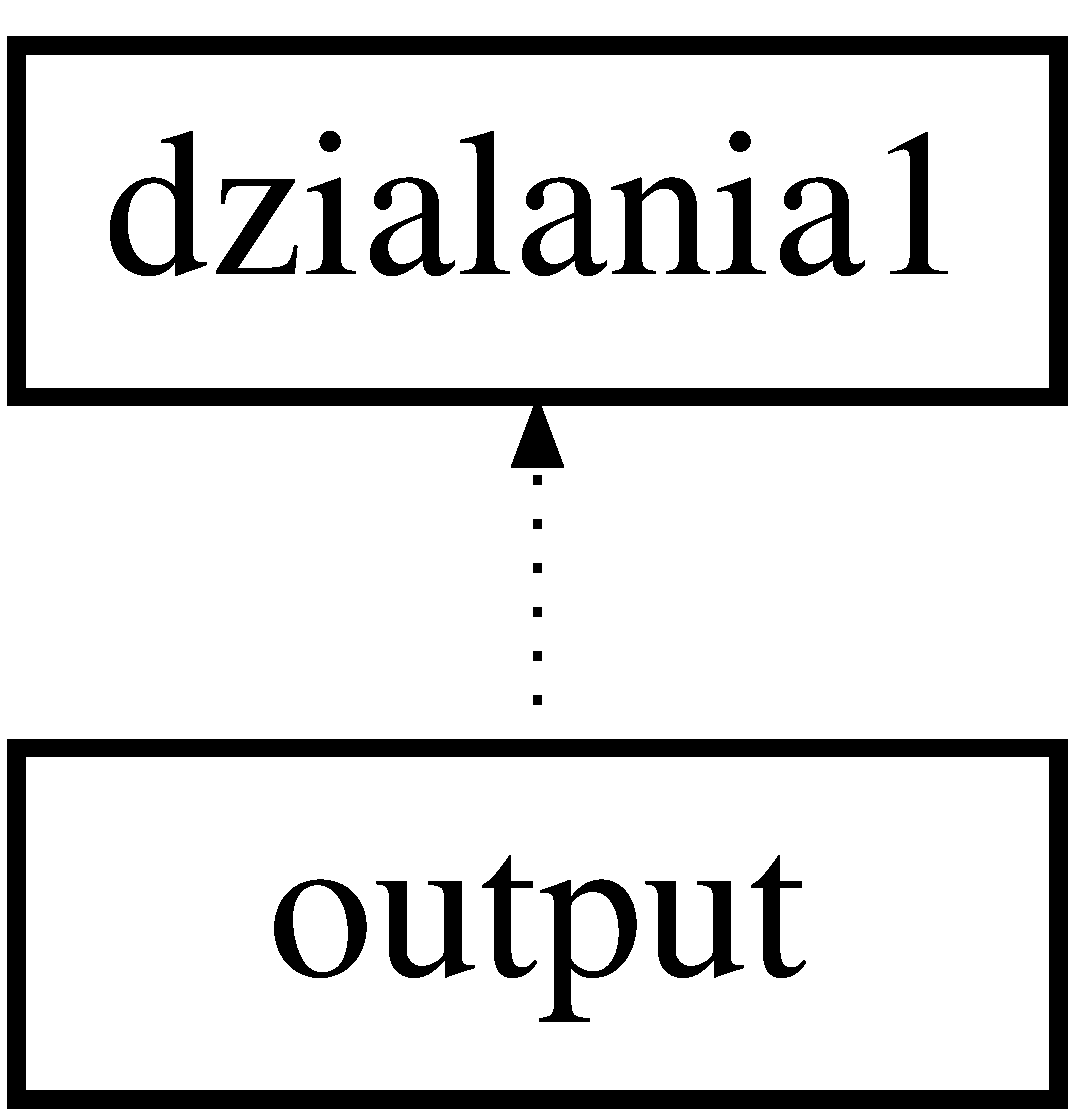
\includegraphics[height=2.000000cm]{classdzialania1}
\end{center}
\end{figure}
\subsection*{Public Member Functions}
\begin{DoxyCompactItemize}
\item 
\hypertarget{classdzialania1_a51de4dbeaa29fc36166d433bf00d4a14}{double {\bfseries mnozenie} (double a, double b)}\label{classdzialania1_a51de4dbeaa29fc36166d433bf00d4a14}

\item 
\hypertarget{classdzialania1_a0eb93a4c85c2236908ba6a1871a4a3b7}{double \hyperlink{classdzialania1_a0eb93a4c85c2236908ba6a1871a4a3b7}{dzielenie} (double a, double b)}\label{classdzialania1_a0eb93a4c85c2236908ba6a1871a4a3b7}

\begin{DoxyCompactList}\small\item\em Funkcja mnozenia. \end{DoxyCompactList}\item 
\hypertarget{classdzialania1_a053b3cc0650eaf81e074c2b3c7501040}{double \hyperlink{classdzialania1_a053b3cc0650eaf81e074c2b3c7501040}{dodawanie} (double a, double b)}\label{classdzialania1_a053b3cc0650eaf81e074c2b3c7501040}

\begin{DoxyCompactList}\small\item\em funkcja dzielenia \end{DoxyCompactList}\item 
\hypertarget{classdzialania1_a333ddbd090054f0ada034fba32f38587}{double \hyperlink{classdzialania1_a333ddbd090054f0ada034fba32f38587}{odejmowanie} (double a, double b)}\label{classdzialania1_a333ddbd090054f0ada034fba32f38587}

\begin{DoxyCompactList}\small\item\em funkcja dodawania \end{DoxyCompactList}\end{DoxyCompactItemize}
\subsection*{Friends}
\begin{DoxyCompactItemize}
\item 
\hypertarget{classdzialania1_a0a8814941837a9542fbb768e740fd03b}{class {\bfseries input}}\label{classdzialania1_a0a8814941837a9542fbb768e740fd03b}

\end{DoxyCompactItemize}


\subsection{Detailed Description}
Klasa \hyperlink{classdzialania1}{dzialania1}. 

Zawiera proste operacje polegajace na dodawaniu, odejmowaniu, mnozeniu, dzieleniu. Obsluguje liczby zmiennoprzecinkowe. 

The documentation for this class was generated from the following file\+:\begin{DoxyCompactItemize}
\item 
Kalkulator.\+cpp\end{DoxyCompactItemize}

\hypertarget{classdzialania2}{\section{dzialania2 Class Reference}
\label{classdzialania2}\index{dzialania2@{dzialania2}}
}


Klasa \hyperlink{classdzialania2}{dzialania2}.  


Inheritance diagram for dzialania2\+:\begin{figure}[H]
\begin{center}
\leavevmode
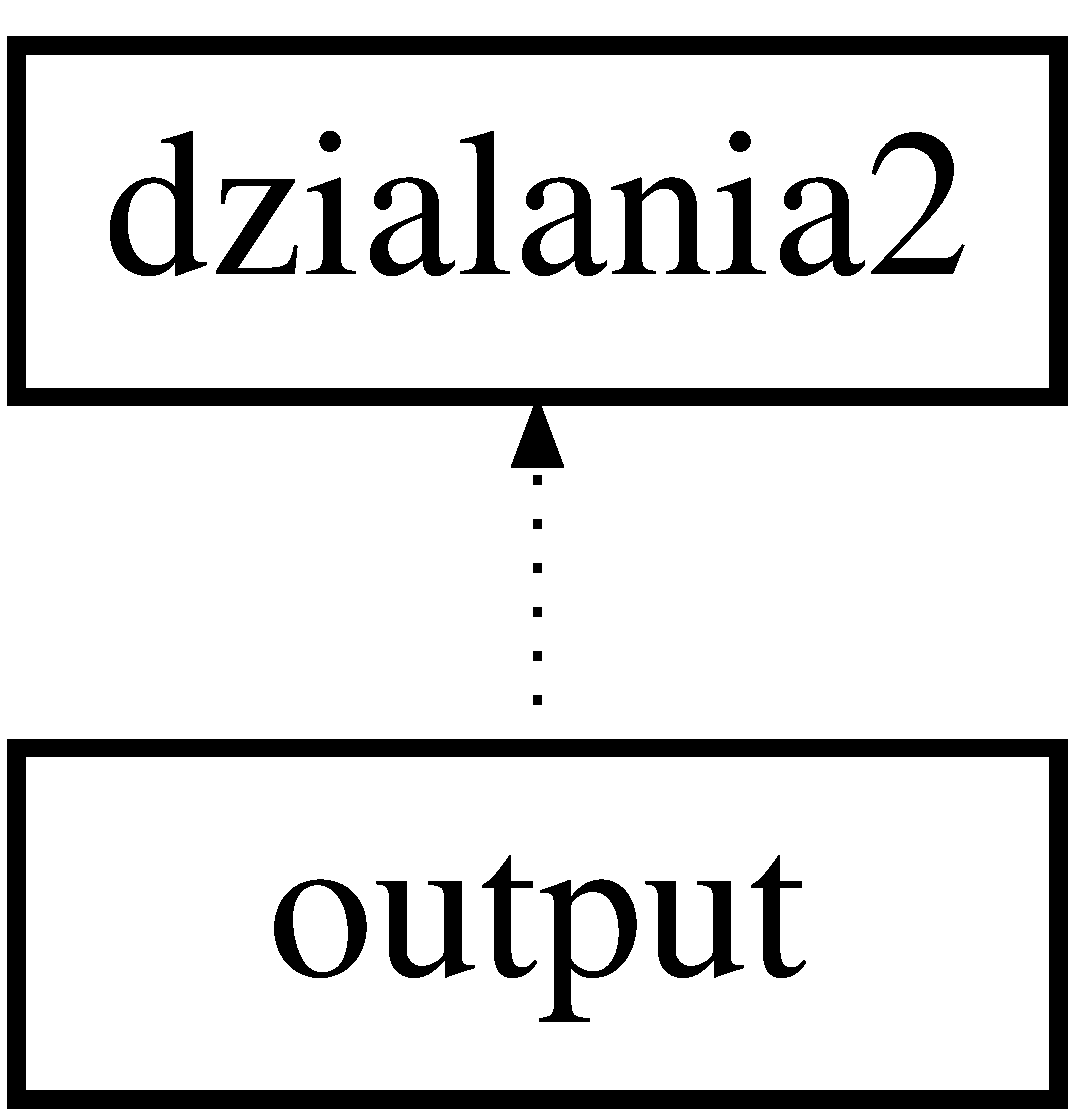
\includegraphics[height=2.000000cm]{classdzialania2}
\end{center}
\end{figure}
\subsection*{Public Member Functions}
\begin{DoxyCompactItemize}
\item 
\hypertarget{classdzialania2_ac5e8b7dbe421513d1d30cf3a79cfa7a4}{double {\bfseries pierwiastek} (double a, double b)}\label{classdzialania2_ac5e8b7dbe421513d1d30cf3a79cfa7a4}

\item 
\hypertarget{classdzialania2_a3223b88f407b20f93b93507d271abe1b}{double \hyperlink{classdzialania2_a3223b88f407b20f93b93507d271abe1b}{potega} (double a, double b)}\label{classdzialania2_a3223b88f407b20f93b93507d271abe1b}

\begin{DoxyCompactList}\small\item\em funkcja pierwiastkowania \end{DoxyCompactList}\end{DoxyCompactItemize}
\subsection*{Friends}
\begin{DoxyCompactItemize}
\item 
\hypertarget{classdzialania2_a0a8814941837a9542fbb768e740fd03b}{class {\bfseries input}}\label{classdzialania2_a0a8814941837a9542fbb768e740fd03b}

\end{DoxyCompactItemize}


\subsection{Detailed Description}
Klasa \hyperlink{classdzialania2}{dzialania2}. 

Zawiera operacje polegajace na pot�gowaniu i pierwiastkowaniu liczb. Obsluguje liczby zmiennoprzecinkowe. 

The documentation for this class was generated from the following file\+:\begin{DoxyCompactItemize}
\item 
Kalkulator.\+cpp\end{DoxyCompactItemize}

\hypertarget{classinput}{\section{input Class Reference}
\label{classinput}\index{input@{input}}
}


Klasa input.  


\subsection*{Public Member Functions}
\begin{DoxyCompactItemize}
\item 
void \hyperlink{classinput_aecd4ecfced6ce24441eead51dcf4456d}{menu} ()
\end{DoxyCompactItemize}


\subsection{Detailed Description}
Klasa input. 

Umo�liwia u�ytkownikowi wyb�r z menu konsolowego poszczegolnych operacji, jak i wpisywanie liczb, do ktorych wynik chce otrzymac. 

\subsection{Member Function Documentation}
\hypertarget{classinput_aecd4ecfced6ce24441eead51dcf4456d}{\index{input@{input}!menu@{menu}}
\index{menu@{menu}!input@{input}}
\subsubsection[{menu}]{\setlength{\rightskip}{0pt plus 5cm}void input\+::menu (
\begin{DoxyParamCaption}
{}
\end{DoxyParamCaption}
)\hspace{0.3cm}{\ttfamily [inline]}}}\label{classinput_aecd4ecfced6ce24441eead51dcf4456d}
zmienne sterujace petlami

zmienne odpowiedzialne za dzialania

obiekt klasy dzialania wyswietlajacy na ekran poprawny wynik

obiekt klasy przelicznik

Petla sterujaca

Umozliwia wybor z menu odpowiedniego dla uzytkownika dzialania

Instrukcja warunkowa Odpowiedzialna za przeniesienie uzytkownika w odpowiednie miejsce programu w zaleznosci od tego jakie operacje chce wykonac

Wybor przez uzytkownika rodzaju przelicznika

Odniesienie do szeregu operacji na liczbach zawartych w klasie dzialania

koniec dzialania programu, wszystkie petle zakonczyly sie prawidlowo. 

The documentation for this class was generated from the following file\+:\begin{DoxyCompactItemize}
\item 
Kalkulator.\+cpp\end{DoxyCompactItemize}

\hypertarget{classoutput}{\section{output Class Reference}
\label{classoutput}\index{output@{output}}
}


Klasa output.  


Inheritance diagram for output\+:\begin{figure}[H]
\begin{center}
\leavevmode
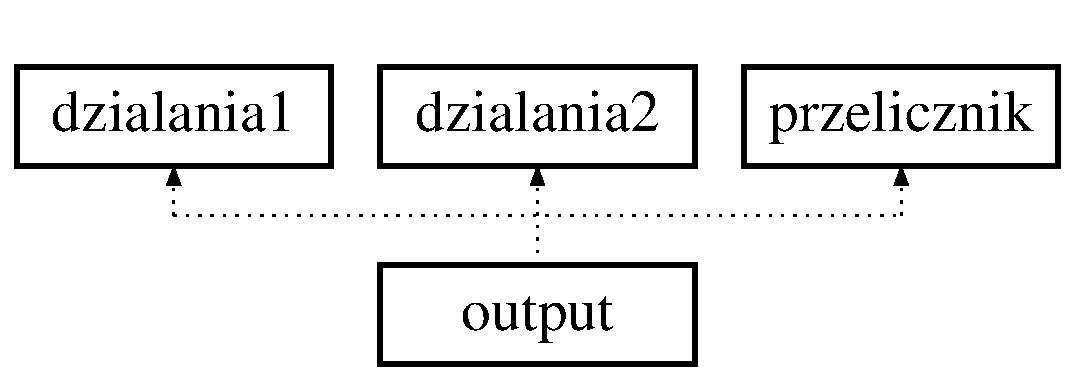
\includegraphics[height=2.000000cm]{classoutput}
\end{center}
\end{figure}
\subsection*{Public Member Functions}
\begin{DoxyCompactItemize}
\item 
\hypertarget{classoutput_a307621f93eddbd31f857bf90dac87f75}{void {\bfseries wyswietl} (double z)}\label{classoutput_a307621f93eddbd31f857bf90dac87f75}

\end{DoxyCompactItemize}
\subsection*{Friends}
\begin{DoxyCompactItemize}
\item 
\hypertarget{classoutput_a0a8814941837a9542fbb768e740fd03b}{class {\bfseries input}}\label{classoutput_a0a8814941837a9542fbb768e740fd03b}

\end{DoxyCompactItemize}


\subsection{Detailed Description}
Klasa output. 

Klasa ta odpowiedzialna jest za wyswietlanie obliczonych wynikow przez kalkulator, przekazuje je uzytkownikowi 

The documentation for this class was generated from the following file\+:\begin{DoxyCompactItemize}
\item 
Kalkulator.\+cpp\end{DoxyCompactItemize}

\hypertarget{classprzelicznik}{\section{przelicznik Class Reference}
\label{classprzelicznik}\index{przelicznik@{przelicznik}}
}


Klasa przelicznik.  


Inheritance diagram for przelicznik\+:\begin{figure}[H]
\begin{center}
\leavevmode
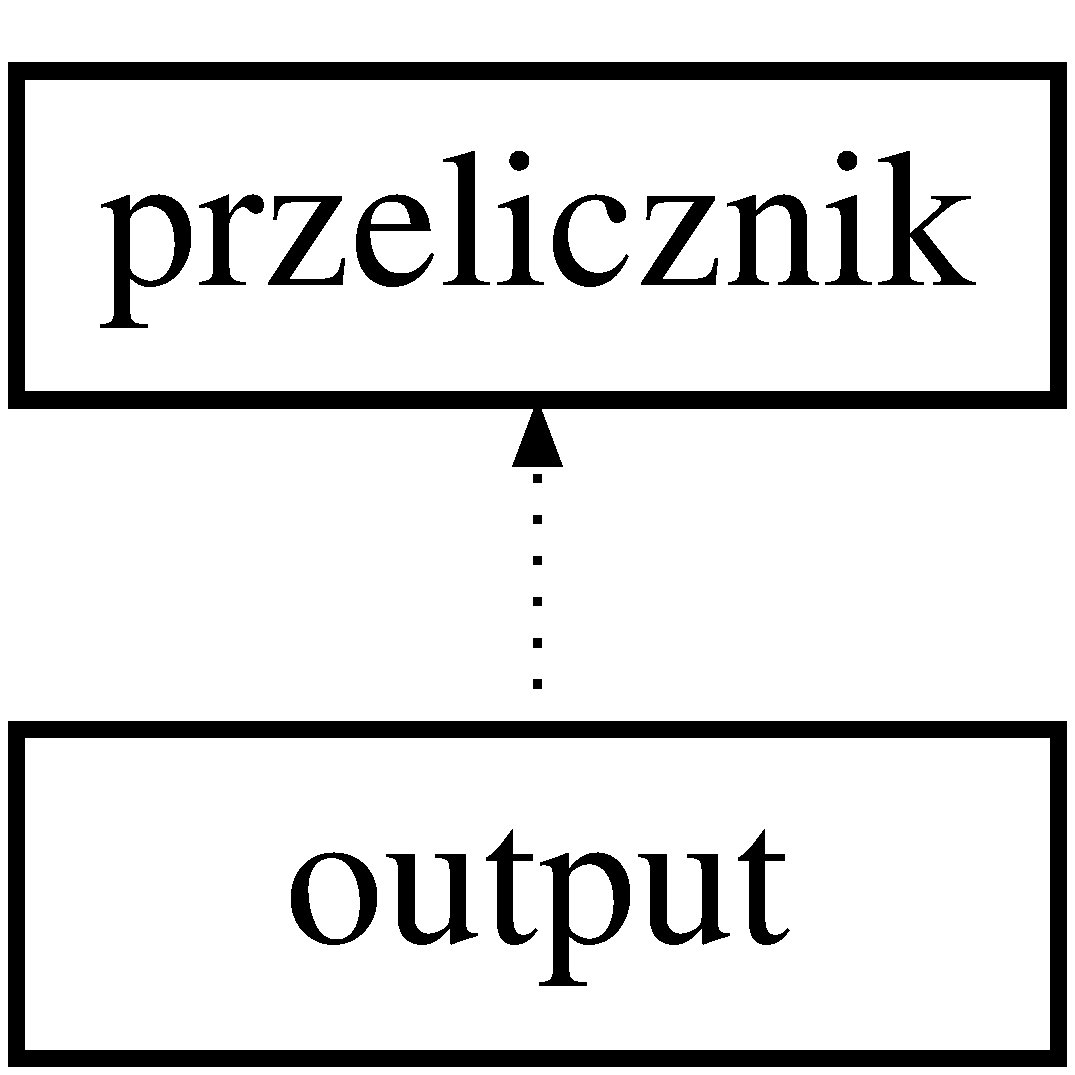
\includegraphics[height=2.000000cm]{classprzelicznik}
\end{center}
\end{figure}
\subsection*{Public Member Functions}
\begin{DoxyCompactItemize}
\item 
\hypertarget{classprzelicznik_af16918bffe6d4e2e45a498a9bb4d7344}{double {\bfseries km\+\_\+mi} (double km)}\label{classprzelicznik_af16918bffe6d4e2e45a498a9bb4d7344}

\item 
\hypertarget{classprzelicznik_a5892f14824367d5a5afe25e01b68fe13}{double {\bfseries mi\+\_\+km} (double mi)}\label{classprzelicznik_a5892f14824367d5a5afe25e01b68fe13}

\end{DoxyCompactItemize}
\subsection*{Public Attributes}
\begin{DoxyCompactItemize}
\item 
\hypertarget{classprzelicznik_acccf8fd1a56dabc8f58237eff8144e36}{double {\bfseries m} = 1.\+609344}\label{classprzelicznik_acccf8fd1a56dabc8f58237eff8144e36}

\end{DoxyCompactItemize}
\subsection*{Friends}
\begin{DoxyCompactItemize}
\item 
\hypertarget{classprzelicznik_a0a8814941837a9542fbb768e740fd03b}{class {\bfseries input}}\label{classprzelicznik_a0a8814941837a9542fbb768e740fd03b}

\end{DoxyCompactItemize}


\subsection{Detailed Description}
Klasa przelicznik. 

Zawiera proste operacje polegajace na zamianie kilometrow na mile oraz mil na kilometry 

The documentation for this class was generated from the following file\+:\begin{DoxyCompactItemize}
\item 
Kalkulator.\+cpp\end{DoxyCompactItemize}

%--- End generated contents ---

% Index
\newpage
\phantomsection
\addcontentsline{toc}{chapter}{Index}
\printindex

\end{document}
